\documentclass[conference,a4paper]{IEEEtran}
\IEEEoverridecommandlockouts

\usepackage{cite}
\usepackage{amsmath,amssymb,amsfonts}
\usepackage{graphicx}
\usepackage{textcomp}
\usepackage{xcolor}
\usepackage{booktabs}
\usepackage{multirow}
\usepackage{subcaption}
\usepackage{url}

\def\BibTeX{{\rm B\kern-.05em{\sc i\kern-.025em b}\kern-.08em
    T\kern-.1667em\lower.7ex\hbox{E}\kern-.125emX}}

\begin{document}

\title{Provider-Aware Contrastive Learning for Accommodation Quality Embeddings in Multi-Provider B2B Travel Platforms}

% Double-blind submission -- author information omitted

\maketitle

\begin{abstract}
Business-to-business (B2B) travel platforms combine accommodation listings from several booking providers. Star ratings in this setting are not directly comparable because each provider applies its own rating scale and data process. We study a contrastive encoder for accommodation quality embeddings on 3.69 million accommodation records from four providers. Positive pairs are sampled from destination--quality-tier groups, and the provider token is masked at inference. The resulting embeddings reduce mean per-dimension cross-provider Kolmogorov--Smirnov (KS) divergence from 0.304 to 0.130 and raise cross-provider nearest-neighbour mixing (CP-NN@10) from 16.7\% to 59.1\%. These results show improved provider mixing, not full provider invariance: provider identity remains recoverable and CP-NN remains below the 75.0\% random-mixing baseline. Short-run provider-removal, CORAL, MMD, and gradient-reversal baselines do not clearly improve CP-NN over stochastic masking.
\end{abstract}

\begin{IEEEkeywords}
contrastive learning, provider invariance, accommodation embeddings, representation learning, B2B travel platforms
\end{IEEEkeywords}

% ---------------------------------------------------------------
\section{Introduction}

Online travel distribution increasingly depends on aggregation. A B2B travel platform may combine accommodation inventory from several booking providers and expose that inventory through banks, agencies, loyalty portals, or other partner channels. Aggregation improves coverage, but it also makes ranking harder because the same field can have different meanings across suppliers.

This paper focuses on accommodation quality signals, especially star ratings. A five-star property from one provider is not necessarily equivalent to a five-star property from another provider. If a ranking system treats provider-native ratings as directly comparable, providers with inflated or differently calibrated ratings may be favored. In our dataset, raw star-rating distributions reach a KS divergence of 0.707 for the most separated provider pair. The data also show an inventory--booking imbalance: one provider contributes 53.7\% of inventory but only 6.4\% of completed transactions. This does not prove that rating mismatch causes lower conversion, but it motivates a representation that is less tied to provider-native rating scales.

The task is therefore narrow: given multi-provider accommodation data without verified cross-provider property links, learn embeddings that preserve useful quality information while reducing provider-specific structure. We train a 128-dimensional contrastive encoder using destination--quality-tier co-membership as weak supervision. At inference, the explicit provider token is set to the masked value.

Prior work gives useful components, but does not directly solve this setting. Huda et al.~\cite{huda2024smart} combine collaborative, demographic, sentiment, and content-based signals for tourism recommendation. Essien et al.~\cite{essien2023deep} review deep-learning applications in hospitality, tourism, and travel. Alamsyah et al.~\cite{alamsyah2019ann} use neural networks for tourism demand forecasting. These papers show the relevance of learning-based methods in travel, but do not study provider rating-scale mismatch inside one aggregated B2B catalogue.

The representation-learning literature motivates the encoder. SimCLR~\cite{chen2020simclr} trains representations from augmented positive views using normalized temperature-scaled cross entropy (NT-Xent). Wang and Isola~\cite{wang2022understanding} describe alignment and uniformity as useful contrastive-learning properties. Gao et al.~\cite{gao2021simcse} show that simple dropout can work as augmentation, and Xia et al.~\cite{yao2021self} use self-supervised graph co-training for recommendation. Khosla et al.~\cite{khosla2020supervised} extend contrastive learning to supervised labels. These methods support the contrastive setup, but they do not address provider-aware accommodation quality.

Domain-invariant learning and calibration are the closest alternatives. Ganin and Lempitsky~\cite{ganin2015unsupervised} use a gradient reversal layer (GRL) to reduce domain separability. Ozyurt et al.~\cite{ozyurt2023cluda} combine contrastive learning with unsupervised domain adaptation. Bai et al.~\cite{bai2024kddebias} study debiasing in recommendation. A simpler option is provider-specific monotonic calibration or ordinal regression with provider offsets~\cite{mccullagh1980regression}. We compare against simple calibration, provider-token removal, covariance alignment (CORAL), maximum mean discrepancy (MMD) alignment, and GRL baselines.

The contributions are: (i) a provider-aware contrastive encoder for accommodation quality embeddings at 3.69M-record scale; (ii) a CP-NN validation protocol for settings without verified cross-provider property identifiers; and (iii) a conservative evaluation showing both alignment gains and remaining provider signal. The rest of the paper describes the data and method, reports baseline comparisons, and discusses limitations.

% ---------------------------------------------------------------
\section{Methods}

\subsection{Data}

We use three datasets from a B2B travel platform. Table~\ref{tab:dataset} summarizes the provider mix. The accommodation metadata contain 3,686,694 property records with provider, star rating, guest rating, popularity score, availability score, price, category, country, destination name, and coordinates. Guest rating is missing for 78.9\% of records. The transaction data contain 3,734 monthly booking-count rows over 13 months. The activity data contain 522,948 tourism listings and are used only for a secondary validation check discussed later.

The implementation and analysis scripts are available at: \url{https://github.com/Liamours/icoict26-challenge-b2b_travel_platform}.

\begin{table}[t]
\caption{Dataset Summary}
\label{tab:dataset}
\begin{center}
\begin{tabular}{lrrl}
\toprule
\textbf{Provider} & \textbf{Inventory} & \textbf{Transactions} & \textbf{Guest Rating} \\
\midrule
RateHawk  & 53.7\% & \phantom{0}6.4\% & Missing \\
Expedia   & 35.4\% & ---              & Available \\
Agoda     & \phantom{0}7.1\% & --- & Available \\
HotelBeds & \phantom{0}3.8\% & 44.2\% & Missing \\
\midrule
Total & \multicolumn{3}{l}{3,686,694 accommodation records} \\
\bottomrule
\end{tabular}
\end{center}
\end{table}

Continuous features are normalized before training. Star ratings are clipped to $[0,5]$, guest ratings to $[0,10]$, coordinates to latitude/90 and longitude/180, and prices are log-transformed after removing values above the 99th percentile. Missing values are represented with binary flags. Provider, category, and country are encoded with learned lookup embeddings.

\subsection{Positive Pairs}

Verified cross-provider property links are not available. We therefore use destination and star-tier co-membership as weak supervision. For property $i$ with star rating $r_i$, the quality tier is
\begin{equation}
t_i=\min\{4,\max\{-1,\lfloor r_i \rfloor\}\},
\label{eq:tier}
\end{equation}
where $\lfloor\cdot\rfloor$ is the floor operator. Missing ratings are assigned to $t_i=-1$ and excluded from positive-pair training. Positive pairs are sampled from the same destination and non-missing tier. With a minimum cluster size of 5, this gives 68,374 valid clusters covering 3,158,693 properties (85.7\%). Coverage is 90.6\%, 85.7\%, and 80.7\% for minimum cluster sizes of 2, 5, and 10, respectively. Cluster sizes are skewed: median 12, p90 80, p99 594, and maximum 22,585.

This supervision is useful but noisy. Two properties in the same city and star tier are not guaranteed to be equivalent. The evaluation therefore treats the learned representation as a provider-mixing embedding, not as verified property matching.

\subsection{Encoder}

The encoder is a compact multilayer perceptron. The input has 43 dimensions: 11 continuous features plus provider, category, and country embeddings of sizes 8, 8, and 16. The hidden layers are 512 and 256 units with batch normalization and ReLU. The stored embedding is 128-dimensional. A projection head maps 128 to 64 to 32 dimensions for contrastive training and is discarded at inference. The encoder has 204,248 trainable parameters.

The dimensions are implementation choices, not claimed optima. A short 20-epoch sweep found that a wider 751k-parameter model increased CP-NN@10 only from 57.4\% to 59.2\%, while increasing model size and provider recoverability. We keep the smaller encoder as a practical trade-off.

\subsection{Training}

The NT-Xent loss uses cosine similarity $s(\cdot,\cdot)$ and temperature $\tau=0.07$~\cite{chen2020simclr}. For a batch with $N=512$ positive pairs, we minimize
\begin{equation}
\mathcal{L}=
-\frac{1}{2N}\sum_{i=1}^{2N}
\log\frac{\exp(s(z_i,z_{j(i)})/\tau)}
{\sum_{k=1}^{2N}\mathbf{1}_{k\neq i}\exp(s(z_i,z_k)/\tau)},
\label{eq:loss}
\end{equation}
where $j(i)$ indexes the paired view of anchor $i$. Augmentation consists of Gaussian noise on continuous features ($\sigma=0.05$), feature dropout (0.2), and provider-token masking with probability 0.5. At inference, the provider token is always masked.

We train with Adam, learning rate $10^{-3}$, weight decay $10^{-6}$, cosine annealing, gradient clipping at 1.0, and early stopping. Because inventory is provider-imbalanced, batches are sampled with equal provider representation.

\subsection{Evaluation}

The main distribution metric is mean per-dimension KS divergence across provider pairs:
\begin{equation}
\mathrm{KS}(X)=\frac{1}{D\binom{|\mathcal{P}|}{2}}\sum_{d=1}^{D}\sum_{p<q}
\sup_x |F_{p,d}(x)-F_{q,d}(x)| ,
\label{eq:ks}
\end{equation}
where $F_{p,d}$ is the empirical CDF for provider $p$ and dimension $d$~\cite{hodges1958significance}. With four providers, the average is over six provider pairs.

The raw baseline uses 13 dimensions: the 11 continuous features plus normalized category and country identifiers, with the provider token excluded. Local provider mixing is measured with CP-NN@K. For query $i$, let $\mathcal{N}_K(i)$ be its $K$ nearest cosine neighbours and $g_i$ its provider:
\begin{equation}
\mathrm{CP\mbox{-}NN@}K=\frac{1}{nK}\sum_{i=1}^{n}\sum_{j\in\mathcal{N}_K(i)}
\mathbf{1}[g_i\neq g_j].
\label{eq:cpnn}
\end{equation}
We use $K=10$ unless stated otherwise. The random-mixing baseline is
\begin{equation}
1-\sum_i p_i^2=0.75,
\label{eq:random}
\end{equation}
where $p_i$ is the provider proportion. Confidence intervals for KS and CP-NN are computed from 30 balanced evaluation resamples, not from independent retraining runs.

% ---------------------------------------------------------------
\section{Results}

\subsection{Main Alignment Results}

Table~\ref{tab:main_results} gives the main comparison. Raw features have low cross-provider mixing: CP-NN@10 is 16.7\%. Simple star calibration does not solve the problem; it slightly lowers KS but also lowers CP-NN. The contrastive embedding reduces KS from 0.304 to 0.130 and raises CP-NN@10 to 59.1\%. It remains below the 75.0\% random baseline, so the result should be read as reduced provider structure, not full invariance.

\begin{table*}[t]
\caption{Main Alignment and Baseline Results}
\label{tab:main_results}
\begin{center}
\begin{tabular}{lccccc}
\toprule
\textbf{Method} & \textbf{KS}~$\downarrow$ & \textbf{Quality Acc.}~$\uparrow$ & \textbf{Provider Acc.}~$\downarrow$ & \textbf{CP-NN@10}~$\uparrow$ & \textbf{Notes} \\
\midrule
Raw features & 0.304 [0.299, 0.309] & 86.2\% & 84.2\% & 16.7\% & 13D feature baseline \\
Star calibration & 0.289 [0.285, 0.295] & -- & 91.3\% & 11.7\% & Provider-wise quantile mapping \\
Provider token removed & -- & 99.1\% & 85.6\% & 57.9\% & Provider always masked during training \\
CORAL penalty & -- & 99.2\% & 84.3\% & 57.9\% & Best of $\lambda\in\{0.01,0.05\}$ \\
MMD penalty & -- & 99.3\% & 85.7\% & 58.2\% & Best of $\lambda\in\{0.01,0.05\}$ \\
GRL baseline & -- & 99.3\% & \textbf{82.9\%} & 58.4\% & Linear schedule, best CP-NN \\
\textbf{Proposed encoder} & \textbf{0.130 [0.124, 0.134]} & \textbf{99.5\%} & 84.0\% & \textbf{59.1\%} & Stochastic provider masking \\
\midrule
Random mixing & -- & -- & -- & 75.0\% & Based on provider proportions \\
\bottomrule
\end{tabular}
\end{center}
\end{table*}

The quality-tier probe reaches 99.3--99.5\% across contrastive variants. This is only a sanity check because tier is also used to construct positive pairs. The more important question is whether provider information is reduced. On the main probe, provider accuracy remains 84.0\%, so provider identity is still recoverable. On a separate balanced 4,000-property masked-inference sample, provider accuracy drops from 84.2\% on raw features to 52.3\% on embeddings; this shows reduced provider signal in that setting, but it does not remove the residual full-space separability seen in the main probe.

The additional distribution metrics point in the same direction. On the balanced validation sample, provider-classifier AUC drops from 0.957 on raw 13-dimensional features to 0.775 on embeddings. Mean MMD$^2$ decreases from 0.414 to 0.037, and mean one-dimensional Wasserstein distance decreases from 0.178 to 0.015. Fig.~\ref{fig:robustness} shows the resampled KS and CP-NN intervals.

\begin{figure}[t]
\centering
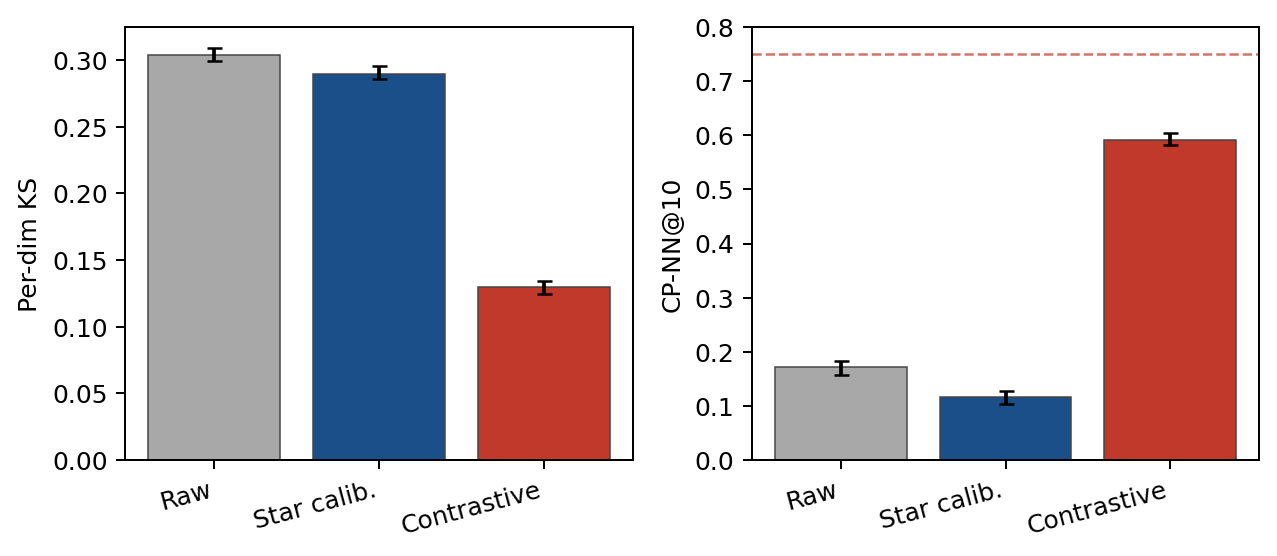
\includegraphics[width=\columnwidth]{figures/reviewer_robustness.png}
\caption{Robustness checks with 95\% intervals from 30 balanced resamples. Left: per-dimension KS. Right: CP-NN@10.}
\label{fig:robustness}
\end{figure}

\subsection{Ablations and Sensitivity}

The provider-token ablation is informative. Training with the provider token always removed gives 57.9\% CP-NN@10, below the proposed stochastic masking result of 59.1\%. This suggests that occasional provider visibility during training is not the main reason for provider mixing; the contrastive destination--tier objective and balanced sampling also matter.

Alignment penalties also do not clearly improve the result. CORAL reaches 57.9\% CP-NN@10 and MMD reaches 58.2\%. At the GRL setting with best CP-NN@10, provider accuracy is 82.9\% and CP-NN@10 is 58.4\%. A stronger GRL setting ($\lambda=0.5$) lowers quality accuracy to 97.7\%, showing the expected utility--invariance trade-off.

CP-NN is stable across neighbourhood sizes. For $K=\{1,5,10,20,50\}$, the proposed embeddings reach 48.3\%, 56.1\%, 59.1\%, 61.8\%, and 64.2\%. Raw features reach 13.9\%, 15.9\%, 16.7\%, 17.7\%, and 19.6\%. With cosine-distance thresholds of 0.05, 0.10, 0.20, and 0.40, embedding CP-NN@10 remains 58.1\%, 59.0\%, 59.1\%, and 59.1\%.

Segment checks show that mixing is not uniform. CP-NN@10 is 63.3\%, 62.0\%, and 60.1\% for small, medium, and large destination-size bands. By price band, it is 51.1\%, 43.4\%, and 55.6\% for low, mid, and high prices. The lower mid-price result suggests that provider-correlated price structure remains.

\subsection{Transaction and Activity Checks}

The transaction data are too sparse for a reliable ranking metric. A conservative audit finds only 13 destinations with at least 10 matched properties and at least 3 booked properties, below the 20-destination threshold set before reporting NDCG. The 40.4\% match rate between transaction and accommodation property identifiers further limits coverage. We therefore do not report NDCG, click-through rate, conversion, or revenue.

The activity-affinity module is also treated as exploratory. A geography-only top-20 baseline retrieves same-destination activities for 98.5\% of destinations, while the learned affinity retrieves same-destination activities at 6.7\% on average. This result argues against using the activity module as evidence for recommendation quality. We keep it only as a future direction.

% ---------------------------------------------------------------
\section{Discussion}
\label{sec:discussion}

The main result is a better provider-mixing representation, not a provider-free representation. KS decreases by 57.4\%, CP-NN@10 rises from 16.7\% to 59.1\%, and MMD/Wasserstein distances also improve. At the same time, provider identity remains recoverable and CP-NN remains below the random baseline. These statements are not contradictory: KS measures marginal one-dimensional alignment, while a provider classifier can use higher-dimensional structure. A raw-feature permutation check also shows that guest-rating missingness, popularity, star-rating missingness, and price missingness carry provider signal.

The positive-pair proxy is the largest methodological limitation. Destination--tier co-membership is available at scale, but it is not the same as verified cross-provider equivalence. Large destination-tier clusters may contain many non-equivalent properties. Future work should use verified property links, entity-resolution models, or manually checked pairs to measure whether local neighbours are truly substitutable.

The baseline results are useful because they narrow the claim. Provider removal, CORAL, MMD, and GRL variants do not clearly beat stochastic masking on CP-NN in short-run experiments. GRL can reduce provider accuracy, but stronger settings begin to reduce quality accuracy. A more complete study should still include longer adversarial training, ordinal calibration with provider offsets, and multiple retraining seeds.

The current evaluation is representation-level. This is appropriate for cold-start inventory, where booking data are sparse, but it does not prove marketplace impact. The transaction audit does not support a reliable NDCG estimate, and the activity module fails against a simple geography baseline. As an operational insight, the embedding is most suitable as an additional ranking or retrieval feature for provider-mixed inventory, not as a direct replacement for booking-based ranking. Deployment would need ranking experiments, drift monitoring, and checks that reducing provider signal does not remove legitimate provider-specific information such as data freshness or coverage quality.

% ---------------------------------------------------------------
\section{Conclusion}

We trained a provider-aware contrastive encoder for accommodation quality embeddings on 3.69 million records. The embedding reduces mean per-dimension KS divergence from 0.304 to 0.130 and raises CP-NN@10 from 16.7\% to 59.1\%. These gains hold across neighbourhood sizes and are not matched by simple calibration, provider-token removal, CORAL, MMD, or short-run GRL baselines. The method remains only partially provider-invariant, and the paper does not claim downstream ranking improvement. The next step is evaluation with verified property links or denser transaction labels.

\section*{Acknowledgment}
The authors thank the data provider for making the datasets available for this study.

\bibliographystyle{IEEEtran}
\bibliography{refs}

\end{document}
